\begin{question}
\noindent Shape A and shape B are drawn on the grid below.

\begin{center}
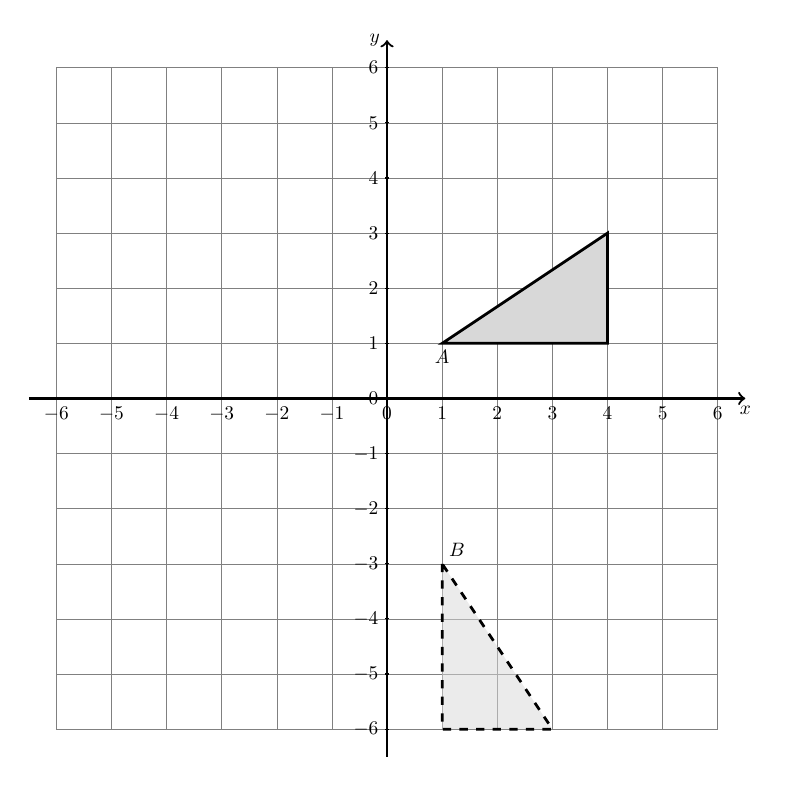
\begin{tikzpicture}[scale=0.7, transform shape]
    \def\axisLimit{6}

    \definecolor{borderColour}{HTML}{000000}
    \definecolor{fillColour}{HTML}{D8D8D8}

    % Grid
    \draw[step=1cm,gray,very thin] (-\axisLimit,-\axisLimit) grid (\axisLimit,\axisLimit);

    % Axes
    \draw[thick,->] (-\axisLimit-0.5,0) -- (\axisLimit+0.5,0) node[anchor=north] {$x$};
    \draw[thick,->] (0,-\axisLimit-0.5) -- (0,\axisLimit+0.5) node[anchor=east] {$y$};

    \foreach \x in {-\axisLimit,...,\axisLimit}
        \draw (\x cm,1pt) -- (\x cm,-1pt) node[anchor=north] {$\x$};
    \foreach \y in {-\axisLimit,...,\axisLimit}
        \draw (1pt,\y cm) -- (-1pt,\y cm) node[anchor=east] {$\y$};

    % Shape A vertices
    \coordinate (A1) at (1,1);
    \coordinate (A2) at (4,1);
    \coordinate (A3) at (4,3);

    \filldraw[fill=fillColour, draw=borderColour, line width=1pt] (A1) -- (A2) -- (A3) -- cycle;
    \node[below] at (A1) {$A$};

    % Shape B vertices: image of A under rotation 90 clockwise about (1,-1)
    \coordinate (B1) at (1,-3);
    \coordinate (B2) at (1,-6);
    \coordinate (B3) at (3,-6);

    \filldraw[fill=fillColour, draw=borderColour, line width=1pt, dashed, fill opacity=0.5] (B1) -- (B2) -- (B3) -- cycle;
    \node[above right] at (B1) {$B$};

\end{tikzpicture}
\end{center}

\begin{enumerate}
    \item[(a)] Find the type of transformation that maps shape A onto shape B.

    \vspace{1.5cm}
    \answerplain{1}

    \item[(b)] Fully describe the single transformation that maps shape A onto shape B.

    \vspace{5cm}
    \answerlines{3}{3}
\end{enumerate}
\end{question}
